\section{Results}
The development of the bird classifier using cased-based reasoning has
been successful in many ways. The final version met all the initial requirements
stated at the beginning of the project and the code has a low footprint while
providing an adequate performance. The leave-one-out-bird cross-validation method has been used
for the validation of the CBR. In details, for validation of the CBR another audio recording
of a bluethroat bird (called bluethroat2) has been added and validated against the database.
Since the database already includes features from bluethroat, a valid classification is expected.

In Figure~\ref{fig:results1} and other figures in this section, we see number of matches over number of
neighbours when comparing 137 samples or 4 seconds of Bluethroat2 against the database. Different figures
represent different weight and distance function configurations.


\begin{figure}[htp]
    \subfloat[Canberra. \fontfamily{qcr}\selectfont \newline 1.0 * FFT Peak 1]{
      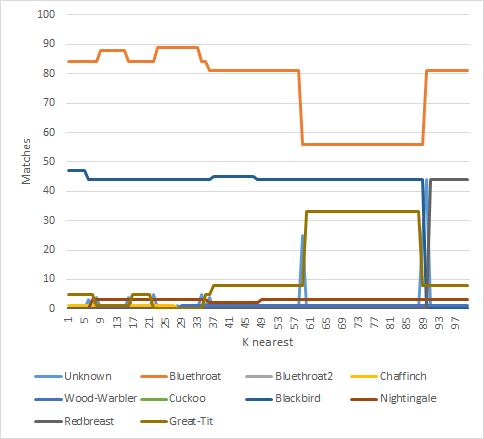
\includegraphics[clip,width=0.4\columnwidth]{eval-canberra-0_0-0_0-1_0-0_0-0_0-0_0-0_0-0_0}
    }
    ~
    \subfloat[Canberra. \fontfamily{qcr}\selectfont \newline 1.0 * FFT Peak 1 \newline 1.0 * FFT Peak 1 Delta]{
      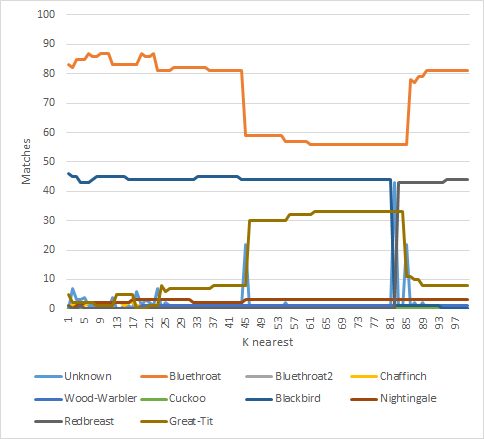
\includegraphics[clip,width=0.4\columnwidth]{eval-canberra-0_0-0_0-1_0-0_0-1_0-0_0-0_0-0_0}
    }
    \caption{Comparing 137 samples or 4 seconds of Bluethroat2 against the database. X-axis is the number of nearest neighbours (the k value) and Y-axis is number of matches for each class of bird.
    This shows adding FFT Peak 1 Delta does not yield significantly better result.  }
    \label{fig:results1}
\end{figure}

\begin{figure}[htp]

  \subfloat[Canberra. \fontfamily{qcr}\selectfont \newline 0.1 * FFT Area Delta. \newline 1.0 * FFT Peak 1 Delta]{
    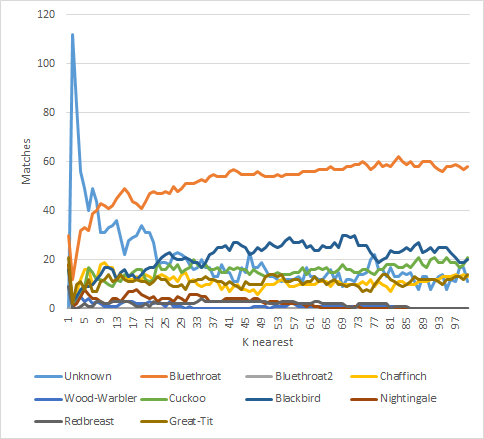
\includegraphics[clip,width=0.4\columnwidth]{eval-canberra-0_0-0_1-0_0-0_0-1_0-0_0-0_0-0_0}
  }
  ~
  \subfloat[Canberra. \fontfamily{qcr}\selectfont \newline 1.0 * FFT Area Delta. \newline 1.0 * FFT Peak 1 Delta]{
    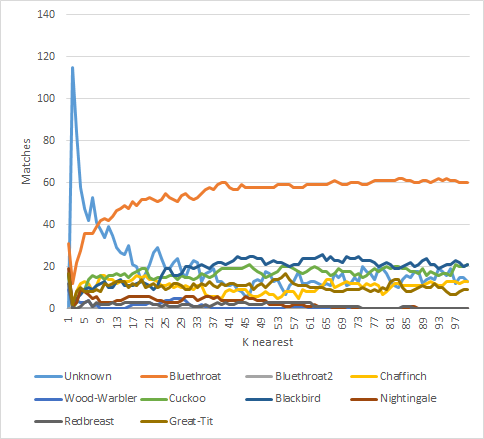
\includegraphics[clip,width=0.4\columnwidth]{eval-canberra-0_0-1_0-0_0-0_0-1_0-0_0-0_0-0_0}
  }
    \caption{This shows a good combination of weights. Note that FFT Peak 1 Delta is necessary.}
    \label{fig:results2}
\end{figure}



\begin{figure}[htp]
    \subfloat[Canberra. \fontfamily{qcr}\selectfont \newline 1.0 * FFT Peak 1 Delta]{
      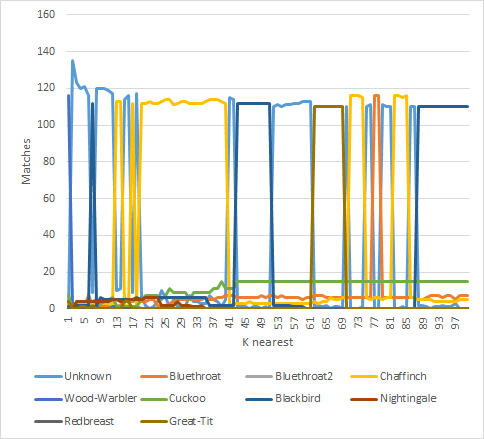
\includegraphics[clip,width=0.4\columnwidth]{eval-canberra-0_0-0_0-0_0-0_0-1_0-0_0-0_0-0_0}
    }
    \caption{Note that FFT Peak 1 Delta alone does not yield acceptable result.}
    \label{fig:results3}
\end{figure}




\begin{figure}[htp]
    \subfloat[Canberra. \fontfamily{qcr}\selectfont \newline 1.0 * FFT Area Delta \newline 0.1 * FFT Peak 1]{
      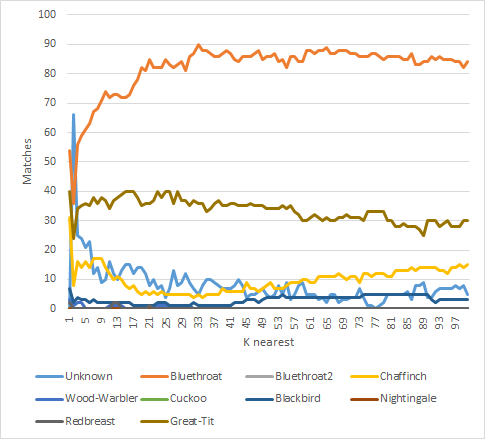
\includegraphics[clip,width=0.4\columnwidth]{eval-canberra-0_0-1_0-0_1-0_1-1_0-0_0-0_0-0_0}
    }
    ~
    \subfloat[Canberra. \fontfamily{qcr}\selectfont \newline 1.0 * FFT Area Delta \newline 1.0 * FFT Peak 1]{
      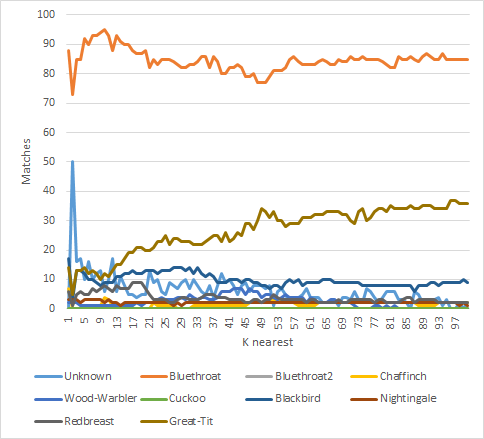
\includegraphics[clip,width=0.4\columnwidth]{eval-canberra-0_0-1_0-1_0-0_0-0_0-0_0-0_0-0_0}
    }

    \subfloat[Canberra. \fontfamily{qcr}\selectfont \newline 1.0 * FFT Area Delta \newline 1.0 * FFT Peak 1  \newline 1.0 * Peak 1 Delta]{
      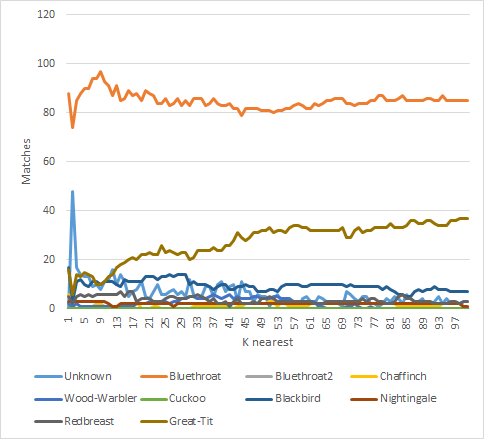
\includegraphics[clip,width=0.4\columnwidth]{eval-canberra-0_0-1_0-1_0-0_0-1_0-0_0-0_0-0_0}
    }
    \caption{}
    \label{fig:results4}
\end{figure}


\begin{figure}[htp]
    \subfloat[Canberra. \fontfamily{qcr}\selectfont \newline 1.0 * FFT Area \newline 1.0 * FFT Area Delta \newline 1.0 * Peak 1 \newline 1.0 * Peak 2 \newline 1.0 * Peak 1 Delta]{
       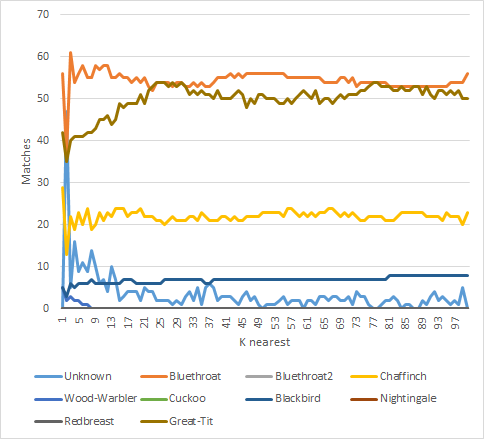
\includegraphics[clip,width=0.4\columnwidth]{eval-canberra-1_0-1_0-1_0-1_0-1_0-0_0-0_0-0_0}
    }
    ~
    \subfloat[Euclidean. \fontfamily{qcr}\selectfont \newline 1.0 * FFT Area \newline 1.0 * FFT Area Delta \newline 1.0 * Peak 1 \newline 1.0 * Peak 2 \newline 1.0 * Peak 1 Delta]{
      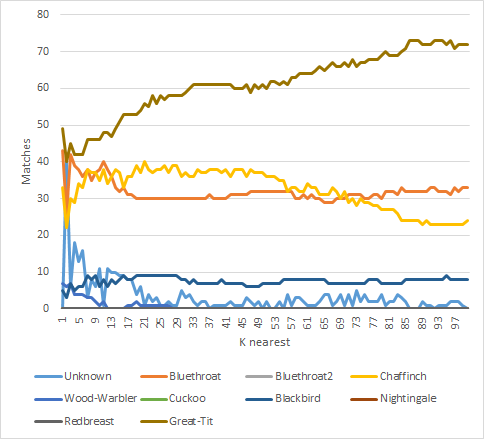
\includegraphics[clip,width=0.4\columnwidth]{eval-euclidean-1_0-1_0-1_0-1_0-1_0-0_0-0_0-0_0}
    }

    \subfloat[Euclidean. \fontfamily{qcr}\selectfont \newline 1.0 * FFT Area \newline 1.0 * FFT Area Delta \newline 1.0 * Peak 1 \newline 1.0 * Peak 2 \newline 1.0 * Peak 1 Delta \newline 1.0 * Mean \newline 1.0 * STD]{
      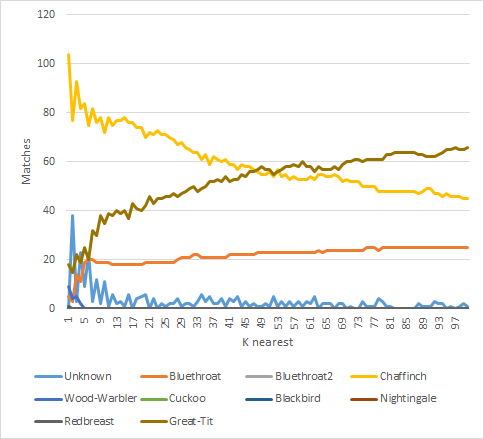
\includegraphics[clip,width=0.4\columnwidth]{eval-euclidean-1_0-1_0-1_0-1_0-1_0-1_0-1_0-0_0}
    }
    \caption{}
    \label{fig:results5}
\end{figure}

\begin{figure}[htp]
    \subfloat[Euclidean. \fontfamily{qcr}\selectfont \newline 1.0 * FFT Area \newline 1.0 * FFT Area Delta \newline 1.0 * Peak 1 \newline 1.0 * Peak 2 \newline 1.0 * Peak 1 Delta \newline 1.0 * Mean \newline 1.0 * STD \newline 1.0 * ZCR]{
      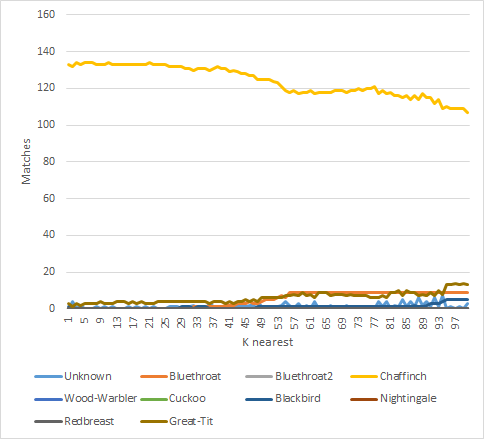
\includegraphics[clip,width=0.4\columnwidth]{eval-euclidean-1_0-1_0-1_0-1_0-1_0-1_0-1_0-1_0}
    }
    ~
    \subfloat[Canberra. \fontfamily{qcr}\selectfont \newline 1.0 * FFT Area \newline 1.0 * FFT Area Delta \newline 1.0 * Peak 1 \newline 1.0 * Peak 2 \newline 1.0 * Peak 1 Delta \newline 1.0 * Mean \newline 1.0 * STD \newline 1.0 * ZCR]{
      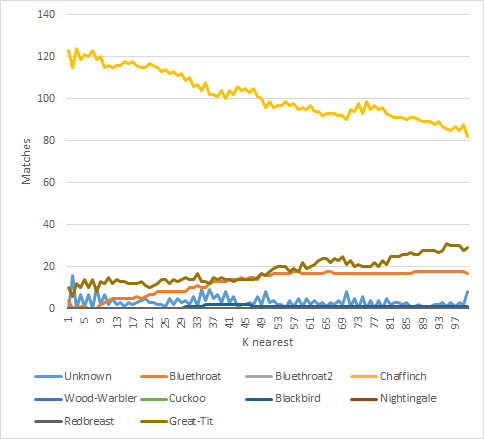
\includegraphics[clip,width=0.4\columnwidth]{eval-canberra-1_0-1_0-1_0-1_0-1_0-1_0-1_0-1_0}
    }

    \subfloat[Manhattan. \fontfamily{qcr}\selectfont \newline 1.0 * FFT Area \newline 1.0 * FFT Area Delta \newline 1.0 * Peak 1 \newline 1.0 * Peak 2 \newline 1.0 * Peak 1 Delta]{
      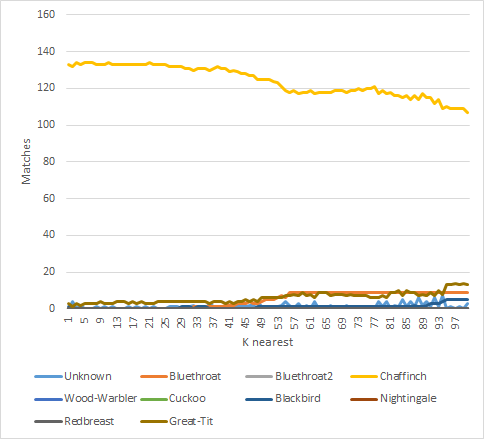
\includegraphics[clip,width=0.4\columnwidth]{eval-manhattan-1_0-1_0-1_0-1_0-1_0-0_0-0_0-0_0}
    }
    \caption{}
    \label{fig:results6}
\end{figure}

The test has showed that it is possable to classify a noisy, different audio strength Bluethroat2 compared to a database with no noize and high quality audio sounded birds.

The tests shows that using Euclidian and Manhattan distance does not yield to accurate results.
The most accurate result were achieved by using the Canberra distance function with different
weight configurations. List of proposed configurations which yield high accuracy include:
\begin{itemize}
  \item Configuration 1: Canberra, 1.0 * FFT Peak 1 Delta, 1.0 * FFT Area Delta.
  \item Configuration 2: Canberra, 1.0 * FFT Peak 1.
  \item Configuration 3: Canberra, 1.0 * FFT Peak 1, 1.0 * FFT Area Delta.
  \item Configuration 4: Canberra, 1.0 * FFT Area Delta, 0.2 * FFT Peak 1, 0.1 * FFT Peak 2, 1.0 * FFT Peak 1 Delta
\end{itemize}

These configurations are found by trial and error and therefore, better configurations may exist.

\section{Discussion}
Configuration number four is currently the best mean accuracy over K from 1 to 100.
Some features can not act alone while others, for example FFT Peak 1 can produce a high accuracy.
When FFT Peak 1 is combined with other features the result will improve if the
weight is decreased for FFT Peak 1. This conclude that that a dominating feature
like FFT Peak 1 may not be that important. It is important not to get biased for
a feature even if that feature alone gives better result than the others.
